\documentclass[11pt, oneside]{article} 
\usepackage{geometry}
\geometry{letterpaper} 
\usepackage{graphicx}
	
\usepackage{amssymb}
\usepackage{amsmath}
\usepackage{parskip}
\usepackage{color}
\usepackage{hyperref}

\graphicspath{{/Users/telliott_admin/Dropbox/Tex/png/}}
% \begin{center} 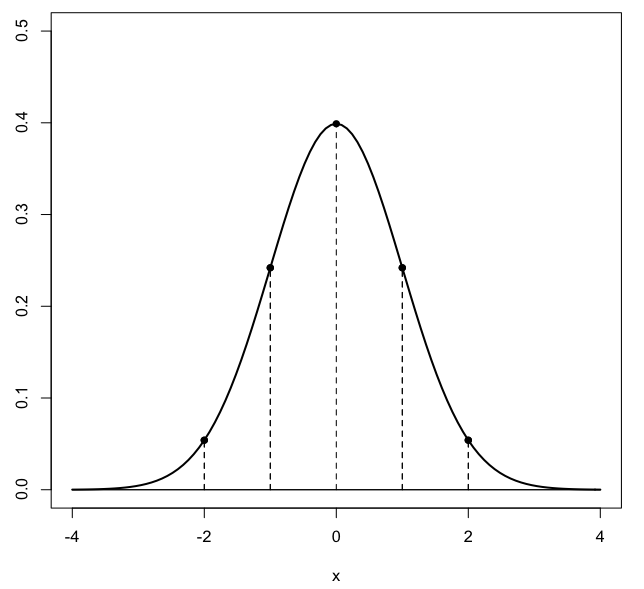
\includegraphics [scale=0.4] {gauss3.png} \end{center}

\title{Trigonometric inverse and hyperbolic functions}
\date{}

\begin{document}
\maketitle
\Large

The hyperbolic functions are defined to be:
\[ 2 \cosh x = e^{x} +  e^{-x}  \]
\[ 2 \sinh x = e^{x} -  e^{-x} \]
\begin{center} 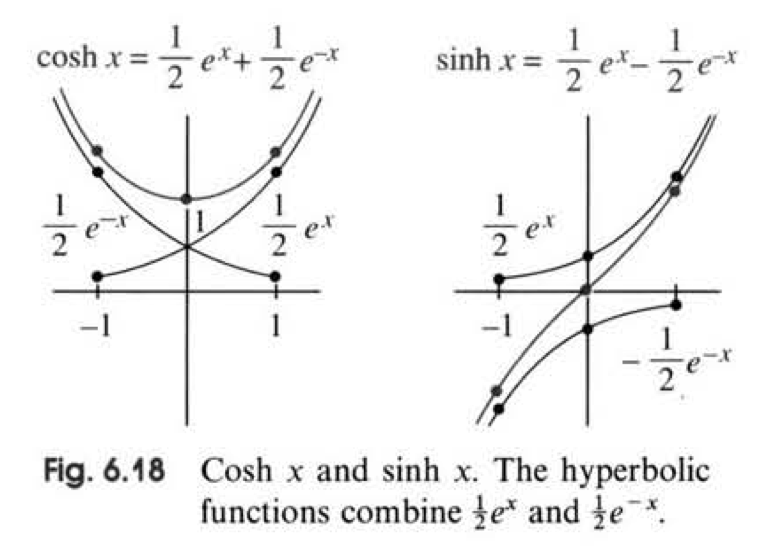
\includegraphics [scale=0.4] {cosh_and_sinh.png} \end{center}

When we work through Euler's formula
\[ e^{ix} = \cos x + i \sin x \]
 we will find that
\[ e^{ix} +  e^{-ix} = 2 \cos x \]
\[ e^{ix} -  e^{-ix} = -2 \ i \sin x \]
which is in a way, parallel to the hyperbolic definitions.

The difference of squares has a simple value:
\[ \cosh^2 t - \sinh^2 t = 1 \]

Everything about the hyperbolic sine is reminiscent of the regular trig functions but with a sign change.

A plot of $\sinh t$ on the x-axis and $\cosh t$ on the y-axis yields a hyperbola in the same way the $y^2 - x^2 = 1$ does.

\subsection*{derivatives}
\[ \frac{d}{dx} 2 \sinh x = \frac{d}{dx} (e^x - e^{-x}) = e^x + e^{-x}  = 2 \cosh x \]
\[ \frac{d}{dx} 2 \cosh x = \frac{d}{dx} (e^x + e^{-x}) = e^x - e^{-x}  = 2 \sinh x \]

Also, note that: 
\[ 2 \sinh x + 2 \cosh x = 2 e^x \]
\[ e^x = \sinh x + \cosh x \]

Because of this, and by symmetry, we expect that the series should be
\[ \sinh x = x + \frac{x^3}{3!} + \frac{x^5}{5!} + \dots \] 
\[ \cosh x = 1 + \frac{x^2}{2!} + \frac{x^4}{4!} + \dots \] 

The values of the functions at zero are
\[ \sinh 0 = 0 \]
\[ \cosh 0 = 1 \]

\subsection*{relativity}
The hyperbolic functions come into the mathematics of relativity, where for an observer in a moving reference frame, the following equations hold:
\[ x' = \frac{x - vt}{\sqrt{1-v^2}} \]
\[ t' = \frac{t - vx}{\sqrt{1-v^2}} \]
The quantity $s^2$ is invariant where
\[ s^2 = t^2 - x^2 \]
Proof:
\[ x'^2 = \frac{x^2 - 2xvt + v^2t^2}{1-v^2} \]
\[ t'^2 = \frac{t^2 - 2xvt + v^2x^2}{1-v^2} \]
\[ t'^2 - x'^2 = \frac{(t^2 - x^2) - v^2(t^2-x^2)}{1-v^2} \]
\[  = t^2 - x^2 \]

The hyperbolic functions come in by defining a parameter $\theta$ (the "rapidity")
\[ \cosh \theta = \frac{1}{\sqrt{1-v^2}} \]
Then
\[ \sinh^2 \theta = \cosh^2 \theta - 1 = \frac{1}{1-v^2} - 1 = \frac{v^2}{1-v^2} \]
\[ \sinh \theta =  \frac{v}{\sqrt{1-v^2}} \]
So we can rewrite
\[ x' = \frac{x - vt}{\sqrt{1-v^2}} = x \cosh \theta - t \sinh \theta \]
\[ t' = \frac{t - vx}{\sqrt{1-v^2}} = t \cosh \theta - x \sinh \theta  \]

\subsection*{$\tanh \theta$}
We had
\[ \sinh \theta =  \frac{v}{\sqrt{1-v^2}} \]
\[ \cosh \theta = \frac{1}{\sqrt{1-v^2}} \]
so 
\[ \tanh \theta = v \]
leading us to explore the properties of the hyperbolic tangent.  Going back to the beginning:
\[ 2 \sinh \theta = e^{\theta} -  e^{-\theta} \]
\[ 2 \cosh \theta = e^{\theta} +  e^{-\theta}  \]
\[ \tanh \theta = \frac{e^{\theta} -  e^{-\theta}}{e^{\theta} +  e^{-\theta}} \]
The derivative is (by the quotient rule):
\[ \frac{d}{d\theta} \ \tanh \theta = \frac{\cosh^2 \theta - \sinh^2 \theta}{\cosh^2 \theta}  \]
\[ =  \frac{1}{\cosh^2 \theta}  \]


\end{document}